\documentclass[10pt,a4paper]{report}

% -----------------------------------------------------------------------------
% PACKAGE IMPORTS
% -----------------------------------------------------------------------------
\usepackage[utf8]{inputenc}
\usepackage[T1]{fontenc}
\usepackage{lmodern}
\usepackage[margin=0.85in,headheight=24pt,top=1in,bottom=1in]{geometry}
\usepackage{amsmath,amssymb}
\usepackage{booktabs}
\usepackage{tabularx}
\usepackage{longtable}
\usepackage{xcolor}
\usepackage{listings}
\usepackage{fancyhdr}
\usepackage{titlesec}
\usepackage{enumitem}
\usepackage{tikz}
\usetikzlibrary{shapes.geometric, arrows.meta, positioning, calc, fit, backgrounds}
\usepackage[skins,breakable]{tcolorbox}
\usepackage{hyperref}

% -----------------------------------------------------------------------------
% COLOR DEFINITIONS & PALETTE
% -----------------------------------------------------------------------------
\definecolor{primaryMaroon}{RGB}{138, 21, 56}     % Baseera primary brand
\definecolor{primaryBlue}{RGB}{20, 52, 100}      % Deep corporate navy
\definecolor{accentGold}{RGB}{212, 160, 23}       % Gold highlight
\definecolor{slateGray}{RGB}{80, 95, 115}        % Neutral slate
\definecolor{lightBg}{RGB}{248, 250, 252}        % Crisp off-white
\definecolor{borderGray}{RGB}{226, 232, 240}      % Soft borders
\definecolor{critRed}{RGB}{185, 28, 28}          % Critical severity
\definecolor{warnOrange}{RGB}{217, 119, 6}       % High / Medium severity
\definecolor{passGreen}{RGB}{22, 101, 52}        % Verified / Low severity
\definecolor{infoBlue}{RGB}{37, 99, 235}         % Informational / Inferred

% -----------------------------------------------------------------------------
% HYPERREF SETUP
% -----------------------------------------------------------------------------
\hypersetup{
    colorlinks=true,
    linkcolor=primaryMaroon,
    filecolor=primaryBlue,
    urlcolor=primaryBlue,
    citecolor=primaryMaroon,
    pdftitle={Baseera -- Full Technical Project Audit Report},
    pdfauthor={Senior Technical Software Auditor},
    pdfsubject={Comprehensive Source Code, Security, and Architectural Audit},
    pdfkeywords={Baseera, Software Audit, React, TypeScript, Groq, LLM, Digital Literacy, Security Review}
}

% -----------------------------------------------------------------------------
% BADGES & MICRO-ELEMENTS
% -----------------------------------------------------------------------------
\newcommand{\verified}{\colorbox{green!15}{\textcolor{passGreen}{\bfseries\scriptsize [VERIFIED]}}}
\newcommand{\inferred}{\colorbox{blue!15}{\textcolor{infoBlue}{\bfseries\scriptsize [INFERRED]}}}
\newcommand{\unknown}{\colorbox{gray!20}{\textcolor{slateGray}{\bfseries\scriptsize [UNKNOWN]}}}

\newcommand{\badgeCrit}{\colorbox{red!20}{\textcolor{critRed}{\bfseries\scriptsize CRITICAL}}}
\newcommand{\badgeHigh}{\colorbox{orange!20}{\textcolor{critRed!80!orange}{\bfseries\scriptsize HIGH}}}
\newcommand{\badgeMed}{\colorbox{yellow!30}{\textcolor{warnOrange!80!black}{\bfseries\scriptsize MEDIUM}}}
\newcommand{\badgeLow}{\colorbox{green!15}{\textcolor{passGreen}{\bfseries\scriptsize LOW}}}

\newcommand{\badgePone}{\colorbox{red!20}{\textcolor{critRed}{\bfseries\scriptsize P1}}}
\newcommand{\badgePtwo}{\colorbox{orange!20}{\textcolor{critRed!80!orange}{\bfseries\scriptsize P2}}}
\newcommand{\badgePthree}{\colorbox{yellow!30}{\textcolor{warnOrange!80!black}{\bfseries\scriptsize P3}}}
\newcommand{\badgePfour}{\colorbox{green!15}{\textcolor{passGreen}{\bfseries\scriptsize P4}}}

\newcommand{\statusPass}{\textcolor{passGreen}{\textbf{Pass}}}
\newcommand{\statusFail}{\textcolor{critRed}{\textbf{Fail}}}
\newcommand{\statusWarn}{\textcolor{warnOrange}{\textbf{Warning}}}

% -----------------------------------------------------------------------------
% TCOLORBOX CALLOUTS
% -----------------------------------------------------------------------------
\newtcolorbox{calloutBox}[2][]{
    colback=lightBg,
    colframe=primaryMaroon,
    coltitle=white,
    fonttitle=\bfseries,
    title=#2,
    arc=2mm,
    boxrule=0.8pt,
    left=3mm, right=3mm, top=2.5mm, bottom=2.5mm,
    breakable,
    #1
}

\newtcolorbox{critBox}[1]{
    colback=red!4!white,
    colframe=critRed,
    coltitle=white,
    fonttitle=\bfseries,
    title=#1,
    arc=2mm,
    boxrule=0.9pt,
    left=3mm, right=3mm, top=2.5mm, bottom=2.5mm,
    breakable
}

\newtcolorbox{warnBox}[1]{
    colback=orange!5!white,
    colframe=warnOrange,
    coltitle=white,
    fonttitle=\bfseries,
    title=#1,
    arc=2mm,
    boxrule=0.8pt,
    left=3mm, right=3mm, top=2.5mm, bottom=2.5mm,
    breakable
}

\newtcolorbox{passBox}[1]{
    colback=green!4!white,
    colframe=passGreen,
    coltitle=white,
    fonttitle=\bfseries,
    title=#1,
    arc=2mm,
    boxrule=0.8pt,
    left=3mm, right=3mm, top=2.5mm, bottom=2.5mm,
    breakable
}

% -----------------------------------------------------------------------------
% LISTINGS STYLING
% -----------------------------------------------------------------------------
\lstset{
    backgroundcolor=\color{lightBg},
    basicstyle=\ttfamily\scriptsize,
    breaklines=true,
    breakatwhitespace=true,
    frame=single,
    rulecolor=\color{borderGray},
    numbers=none,
    keywordstyle=\color{primaryMaroon}\bfseries,
    commentstyle=\color{slateGray}\itshape,
    stringstyle=\color{passGreen},
    showstringspaces=false,
    tabsize=2
}

% -----------------------------------------------------------------------------
% HEADERS & FOOTERS
% -----------------------------------------------------------------------------
\pagestyle{fancy}
\fancyhf{}
\fancyhead[L]{\small\textcolor{slateGray}{\textbf{Baseera} -- Full Technical Project Audit Report}}
\fancyhead[R]{\small\textcolor{slateGray}{\leftmark}}
\fancyfoot[L]{\footnotesize\textcolor{slateGray}{Confidential -- Technical Audit Review}}
\fancyfoot[R]{\footnotesize\textcolor{slateGray}{Page \thepage}}
\renewcommand{\headrulewidth}{0.4pt}
\renewcommand{\headrule}{\hbox to\headwidth{\color{borderGray}\leaders\hrule height \headrulewidth\hfill}}

\definecolor{darkNavy}{RGB}{15, 23, 42}          % Dark navy text

% -----------------------------------------------------------------------------
% TITLE FORMATTING
% -----------------------------------------------------------------------------
\titleformat{\chapter}[display]
  {\normalfont\bfseries\color{primaryMaroon}}
  {\filleft\Huge\color{slateGray}SECTION \thechapter}
  {3ex}
  {\titlerule\vspace{1.5ex}\LARGE}
  [\vspace{1.5ex}\titlerule]

\titleformat{\section}
  {\normalfont\Large\bfseries\color{primaryBlue}}
  {\thesection}{0.8em}{}

\titleformat{\subsection}
  {\normalfont\large\bfseries\color{primaryMaroon!90!black}}
  {\thesubsection}{0.8em}{}

\titleformat{\subsubsection}
  {\normalfont\normalsize\bfseries\color{darkNavy}}
  {\thesubsubsection}{0.8em}{}

% -----------------------------------------------------------------------------
% DOCUMENT BODY
% -----------------------------------------------------------------------------
\begin{document}

% -----------------------------------------------------------------------------
% TITLE PAGE
% -----------------------------------------------------------------------------
\begin{titlepage}
    \centering
    \vspace*{1cm}
    
    {\Huge \bfseries \textcolor{primaryMaroon}{BASEERA} \par}
    \vspace{0.3cm}
    {\LARGE \bfseries \textcolor{primaryBlue}{FULL TECHNICAL PROJECT AUDIT REPORT} \par}
    \vspace{0.4cm}
    {\large \textcolor{slateGray}{Exhaustive, Evidence-Based Codebase Audit \& Engineering Evaluation} \par}
    
    \vspace{1.2cm}
    \rule{\linewidth}{1.5pt}
    \vspace{0.4cm}
    
    \begin{quote}
        \centering
        \itshape\large
        ``Teaching minds to doubt, not machines to decide.''
    \end{quote}
    
    \vspace{0.4cm}
    \rule{\linewidth}{1.5pt}
    \vspace{1.5cm}
    
    \begin{tcolorbox}[colback=lightBg,colframe=primaryMaroon,arc=3mm,width=0.92\linewidth]
        \centering
        \textbf{EXECUTIVE SUMMARY CLASSIFICATION} \\
        \vspace{0.2cm}
        \textcolor{critRed}{\bfseries Working MVP with Critical Architectural and Security Caveats} \\
        \vspace{0.15cm}
        \small All 49 automated tests pass; full client-side React 19 application; \\
        severe API key exposure and mock authentication require immediate remediation prior to production.
    \end{tcolorbox}
    
    \vspace{1.5cm}
    
    \begin{minipage}{0.48\textwidth}
        \begin{flushleft} \small
            \textbf{Project Name:} Baseera (Arabic: insight, vision) \\
            \textbf{Target Domain:} Digital Literacy \& Cognitive Security \\
            \textbf{Audited Release:} 0.0.0 (Hackathon Pre-Release MVP) \\
            \textbf{Context:} Erasmus+ VirtuallyEdu Digital Hackathon \\
            \textbf{Document Type:} Comprehensive Technical Audit
        \end{flushleft}
    \end{minipage}
    \hfill
    \begin{minipage}{0.48\textwidth}
        \begin{flushright} \small
            \textbf{Audit Date:} October 13, 2026 \\
            \textbf{Lead Auditor:} Senior Software Auditor \\
            \textbf{Methodology:} Line-by-Line Code Review \\
            \textbf{Verification Mode:} Empirical \& Evidence-Based \\
            \textbf{Report Status:} Final Complete Audit
        \end{flushright}
    \end{minipage}
    
    \vfill
    {\footnotesize \textcolor{slateGray}{Typeset with \LaTeX\ -- Verified Against Local Codebase \& Live Test Execution}}
\end{titlepage}

% -----------------------------------------------------------------------------
% TABLE OF CONTENTS
% -----------------------------------------------------------------------------
\tableofcontents
\newpage

% =============================================================================
\chapter{Executive Summary}
% =============================================================================

\section{What This Project Is}
\textbf{Baseera} (\textit{Arabic for ``insight'' or ``clear vision''}) is an AI-powered \textbf{Digital Literacy Coach} mobile and web application. It was conceived, designed, and engineered for the \textbf{Erasmus+ VirtuallyEdu Digital Hackathon} by an international five-person student collaboration across Algeria, Armenia, Greece, Ukraine, and Georgia.

The platform targets impulsive viral misinformation propagation. Instead of acting as an automated truth arbiter or appending binary ``True/False'' badges, Baseera introduces an ambient cognitive pause and applies Socratic inquiry to guide users toward questioning emotional tone, urgency manipulation, and missing contextual corroboration before sharing digital content.

\section{Current State: Working MVP with Significant Caveats}
The audited codebase is a functioning prototype:
\begin{itemize}[leftmargin=1.5em]
    \item \textbf{Build and Execution:} The application compiles cleanly with Vite, launches on port 5173, and bundles into a native Android APK via Capacitor.
    \item \textbf{Test Suite:} Vitest executes \textbf{49 unit and integration tests across 3 suites, achieving 100\% pass rate} (duration $\approx$ 30.28s).
    \item \textbf{Critical Caveats:} Severe security vulnerabilities exist, including plaintext API keys committed to source files, client-side key embedding via Vite environment variables, plaintext credential storage in \texttt{localStorage}, and simulated mock implementations for key advertised features (Privacy Shield, Reports).
\end{itemize}

\section{Top 5 Most Important Findings}

\begin{table}[htbp]
\centering
\small
\caption{Executive Priority Findings Matrix}
\begin{tabularx}{\textwidth}{c p{5.5cm} c p{4cm}}
\toprule
\textbf{\#} & \textbf{Finding \& Nature} & \textbf{Severity} & \textbf{Source Evidence} \\
\midrule
1 & \verified\ \textbf{API Keys Hardcoded \& Exposed} \newline Gemini and Groq Cloud production keys hardcoded in root test scripts and \texttt{.env}. & \badgeCrit & \texttt{.env:1-2}, \newline \texttt{test\_gemini.cjs:2}, \newline \texttt{test\_groq.cjs:1} \\
\addlinespace
2 & \verified\ \textbf{Plaintext Password Storage in LocalStorage} \newline Registration and login store raw unhashed passwords directly in browser storage. & \badgeCrit & \texttt{SignupScreen.tsx:41}, \newline \texttt{LoginScreen.tsx:25} \\
\addlinespace
3 & \verified\ \textbf{Privacy Shield Feature Entirely Simulated} \newline advertised facial blurring and EXIF stripping are hardcoded mock UI elements. & \badgeMed & \texttt{PrivacyScreen.tsx:5-9} \\
\addlinespace
4 & \verified\ \textbf{Static Analytics \& Habit Metrics} \newline Weekly habit score (88\%) and charts are hardcoded numbers, not computed from observations. & \badgeMed & \texttt{HomeScreen.tsx:104,116}, \newline \texttt{ReportsScreen.tsx:13-36} \\
\addlinespace
5 & \verified\ \textbf{Unsubstantiated Marketing Claims in UI} \newline Claims of ``280+ peer-reviewed archives'' and ``end-to-end encryption'' have zero implementation. & \badgeHigh & \texttt{ShareScreen.tsx:390,408}, \newline \texttt{ProcessingScreen.tsx:196} \\
\bottomrule
\end{tabularx}
\end{table}

% =============================================================================
\chapter{Project Identity}
% =============================================================================

\begin{table}[htbp]
\centering
\small
\caption{System Identity Specification}
\begin{tabularx}{\textwidth}{l X}
\toprule
\textbf{Property} & \textbf{Value / Specification} \\
\midrule
\textbf{Name} & Baseera (\textit{Arabic: insight, discernment, clear perception}) \\
\textbf{Core Purpose} & AI-assisted digital literacy coach to provoke critical reflection before social sharing \\
\textbf{Target Audience} & Digital citizens, students, educators, and hackathon evaluation panels \\
\textbf{Problem Addressed} & Impulsive sharing of sensationalist, emotionally manipulative misinformation \\
\textbf{Deployment Targets} & Progressive Web App (SPA) + Android APK via Apache Capacitor \\
\textbf{Repository Footprint} & $\approx$ 180 KB source code (excl. node\_modules); 5.9 MB compiled Android APK \\
\textbf{Language Distribution} & TypeScript / TSX ($\approx$ 95\%), CSS ($\approx$ 3\%), HTML ($\approx$ 1\%), Python ($\approx$ 1\% helper tools) \\
\textbf{Project Genesis} & Erasmus+ VirtuallyEdu Digital Hackathon submission \\
\textbf{International Team} & Abdelkader (Algeria, Lead), Azatuhi (Armenia), Fotini (Greece), Anastasia (Ukraine), Milena (Georgia) \\
\textbf{Core Philosophical Motto} & \textit{``Teaching minds to doubt, not machines to decide.''} \\
\bottomrule
\end{tabularx}
\end{table}

% =============================================================================
\chapter{Technology Stack}
% =============================================================================

\begin{table}[htbp]
\centering
\scriptsize
\caption{Full Technology Stack Audit}
\begin{tabularx}{\textwidth}{l l l X p{3.2cm}}
\toprule
\textbf{Layer} & \textbf{Technology} & \textbf{Version} & \textbf{Role \& Placement} & \textbf{Audit Assessment} \\
\midrule
Language & TypeScript & $\sim$6.0.2 & Static type-safety across all \texttt{src/} modules & Modern ES2023 compilation target \\
UI Framework & React & \textasciicircum 19.2.8 & Core component hierarchy & Modern React 19; functional style \\
Client Routing & react-router-dom & \textasciicircum 7.18.4 & Hash/browser client navigation & React Router v7; clean setup \\
Data Visuals & Recharts & \textasciicircum 3.10.1 & Bar graphs in \texttt{ReportsScreen.tsx} & Large bundle footprint for single chart \\
Build Bundler & Vite & \textasciicircum 8.3.0 & Dev HMR server and production packaging & Fast, highly optimized builds \\
Styling Engine & TailwindCSS & \textasciicircum 3.4.19 & Utility CSS with Material Design 3 tokens & Stable v3 line with custom theme \\
PostCSS & postcss/autoprefixer & \textasciicircum 8.5.28 & CSS vendor prefixing & Standard pipeline \\
Mobile Bridge & Capacitor Core/Android & \textasciicircum 8.5.2 & Wraps web assets in native Android WebView & Clean bridge configuration \\
AI Engine & Groq Cloud API & REST & Remote inference via \texttt{qwen/qwen3.8-27b} & Direct client-to-API calls \\
AI SDK (Unused) & @google/generative-ai & \textasciicircum 0.24.1 & Google Gemini SDK & \unknown\ Unused in app; only in test scripts \\
Testing & Vitest & \textasciicircum 5.0.2 & Unit test execution with JSDOM runner & Fast runner; 49 tests passing \\
Test Support & @testing-library/react & \textasciicircum 16.3.3 & DOM integration testing & Standard React testing harness \\
Linter & OxLint & \textasciicircum 1.81.0 & Rust-based static code analyzer & React and TS rules enabled \\
Typography & Google Fonts CDN & Remote & Plus Jakarta Sans and Noto Serif & Requires external connectivity \\
Icons & Material Symbols & Remote & Iconography rendered via span text tags & Loaded from Google CDN \\
\bottomrule
\end{tabularx}
\end{table}

% =============================================================================
\chapter{System Architecture}
% =============================================================================

\section{High-Level Architecture Description}
Baseera is architected as a \textbf{decoupled single-page web application (SPA)} wrapped inside an Apache Capacitor mobile shell. It exhibits a \textbf{Backend-less / Zero-Server topology}:
\begin{itemize}[leftmargin=1.5em]
    \item No custom backend server, database, or proxy middleware is deployed.
    \item State is maintained client-side via in-memory singletons (\texttt{store.ts}) and persistent browser storage (\texttt{localStorage}).
    \item AI inference is executed directly from the user's browser or mobile WebView to Groq Cloud's REST API over HTTPS.
\end{itemize}

\section{Component Architecture Diagram}
Figure~\ref{fig:component_diagram} illustrates the internal component layout and external boundary connections.

\begin{figure}[htbp]
\centering
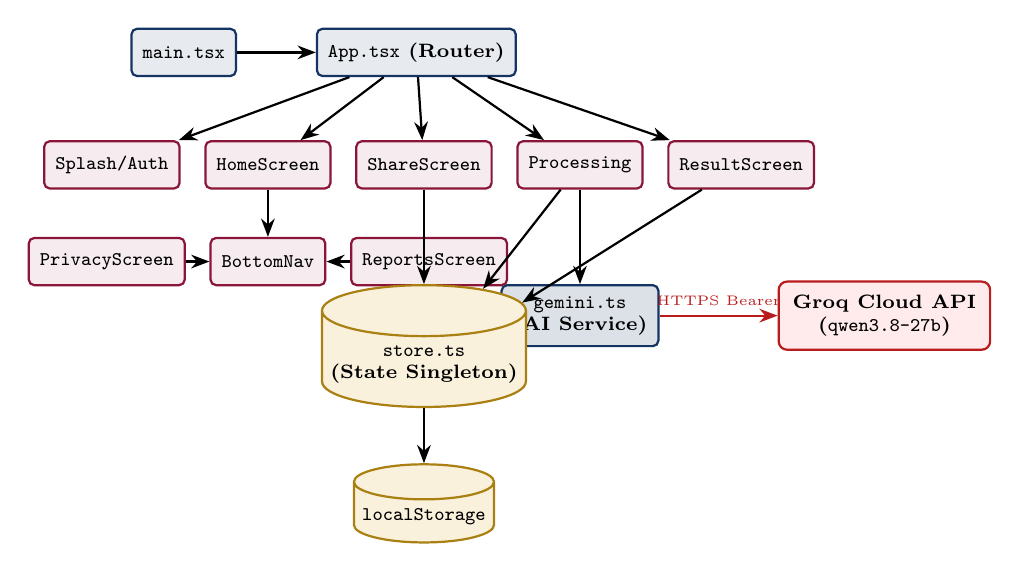
\begin{tikzpicture}[
    node distance=0.8cm and 1.2cm,
    box/.style={rectangle, draw=primaryBlue, fill=lightBg, rounded corners=2pt, thick, align=center, font=\scriptsize\bfseries, inner sep=4pt, minimum height=0.6cm},
    screen/.style={rectangle, draw=primaryMaroon, fill=primaryMaroon!8!white, rounded corners=2pt, thick, align=center, font=\scriptsize, inner sep=4pt, minimum height=0.6cm},
    store/.style={cylinder, shape border rotate=90, draw=accentGold!80!black, fill=accentGold!15!white, aspect=0.25, thick, font=\scriptsize\bfseries, align=center, inner sep=3pt},
    ext/.style={rectangle, draw=critRed, fill=red!8!white, rounded corners=3pt, thick, align=center, font=\scriptsize\bfseries, inner sep=5pt},
    >=Stealth, thick
]

% Client Box
\node[box, fill=primaryBlue!10!white] (main) {\texttt{main.tsx}};
\node[box, fill=primaryBlue!10!white, right=1cm of main] (app) {\texttt{App.tsx} (Router)};

% Screens
\node[screen, below left=0.8cm and -0.2cm of app] (home) {\texttt{HomeScreen}};
\node[screen, left=0.3cm of home] (splash) {\texttt{Splash/Auth}};
\node[screen, right=0.3cm of home] (share) {\texttt{ShareScreen}};
\node[screen, right=0.3cm of share] (proc) {\texttt{Processing}};
\node[screen, right=0.3cm of proc] (res) {\texttt{ResultScreen}};

% Shared Nav & Auxiliary
\node[screen, below=0.6cm of home] (nav) {\texttt{BottomNav}};
\node[screen, left=0.3cm of nav] (priv) {\texttt{PrivacyScreen}};
\node[screen, right=0.3cm of nav] (rep) {\texttt{ReportsScreen}};

% Services & Stores
\node[box, below=1.2cm of proc, fill=primaryBlue!15!white] (ai) {\texttt{gemini.ts} \\ (AI Service)};
\node[store, below=1.2cm of share] (store) {\texttt{store.ts} \\ (State Singleton)};
\node[store, below=0.7cm of store] (ls) {\texttt{localStorage}};

% External
\node[ext, right=1.5cm of ai] (groq) {Groq Cloud API \\ (\texttt{qwen3.8-27b})};

% Edges
\draw[->] (main) -- (app);
\draw[->] (app) -- (splash);
\draw[->] (app) -- (home);
\draw[->] (app) -- (share);
\draw[->] (app) -- (proc);
\draw[->] (app) -- (res);

\draw[->] (home) -- (nav);
\draw[->] (priv) -- (nav);
\draw[->] (rep) -- (nav);

\draw[->] (share) -- (store);
\draw[->] (proc) -- (store);
\draw[->] (proc) -- (ai);
\draw[->] (res) -- (store);
\draw[->] (store) -- (ls);

\draw[->, draw=critRed] (ai) -- node[above, font=\tiny, text=critRed] {HTTPS Bearer} (groq);

\end{tikzpicture}
\caption{Baseera System Component and Communication Architecture}
\label{fig:component_diagram}
\end{figure}

\section{Content Analysis Data Flow}
Figure~\ref{fig:sequence_diagram} documents the end-to-end execution flow when a user analyzes a URL or multimodal image.

\begin{figure}[htbp]
\centering
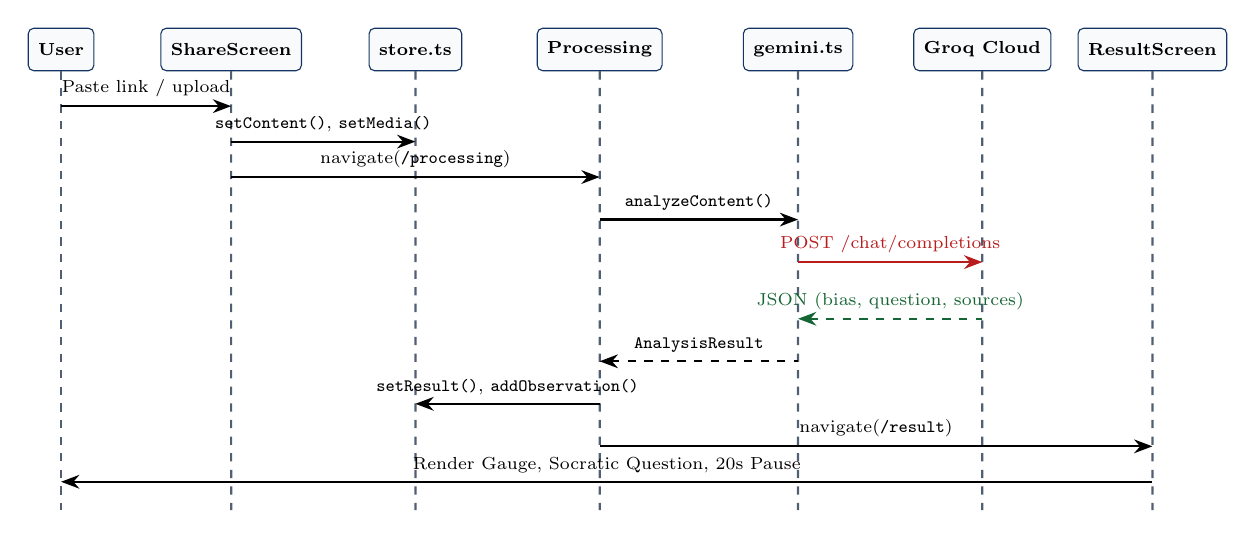
\begin{tikzpicture}[
    scale=0.9, every node/.style={scale=0.9},
    lifeline/.style={draw=slateGray, dashed, thick},
    entity/.style={rectangle, draw=primaryBlue, fill=lightBg, rounded corners=2pt, font=\scriptsize\bfseries, inner sep=4pt, minimum height=0.6cm, align=center},
    msg/.style={->, >=Stealth, thick, font=\scriptsize},
    return/.style={<-, >=Stealth, dashed, thick, font=\scriptsize}
]

\node[entity] (u) at (0,0) {User};
\node[entity] (ss) at (2.4,0) {ShareScreen};
\node[entity] (st) at (5.0,0) {store.ts};
\node[entity] (ps) at (7.6,0) {Processing};
\node[entity] (ai) at (10.4,0) {gemini.ts};
\node[entity] (gq) at (13.0,0) {Groq Cloud};
\node[entity] (rs) at (15.4,0) {ResultScreen};

\draw[lifeline] (u) -- (0,-6.5);
\draw[lifeline] (ss) -- (2.4,-6.5);
\draw[lifeline] (st) -- (5.0,-6.5);
\draw[lifeline] (ps) -- (7.6,-6.5);
\draw[lifeline] (ai) -- (10.4,-6.5);
\draw[lifeline] (gq) -- (13.0,-6.5);
\draw[lifeline] (rs) -- (15.4,-6.5);

% Messages
\draw[msg] (0,-0.8) -- node[above] {Paste link / upload} (2.4,-0.8);
\draw[msg] (2.4,-1.3) -- node[above] {\texttt{setContent()}, \texttt{setMedia()}} (5.0,-1.3);
\draw[msg] (2.4,-1.8) -- node[above] {navigate(\texttt{/processing})} (7.6,-1.8);
\draw[msg] (7.6,-2.4) -- node[above] {\texttt{analyzeContent()}} (10.4,-2.4);

% API Call
\draw[msg, draw=critRed] (10.4,-3.0) -- node[above, text=critRed] {POST /chat/completions} (13.0,-3.0);
\draw[return, draw=passGreen] (10.4,-3.8) -- node[above, text=passGreen] {JSON (bias, question, sources)} (13.0,-3.8);

\draw[return] (7.6,-4.4) -- node[above] {\texttt{AnalysisResult}} (10.4,-4.4);
\draw[msg] (7.6,-5.0) -- node[above] {\texttt{setResult()}, \texttt{addObservation()}} (5.0,-5.0);
\draw[msg] (7.6,-5.6) -- node[above] {navigate(\texttt{/result})} (15.4,-5.6);
\draw[msg] (15.4,-6.1) -- node[above] {Render Gauge, Socratic Question, 20s Pause} (0,-6.1);

\end{tikzpicture}
\caption{End-to-End Content Analysis Sequence Execution}
\label{fig:sequence_diagram}
\end{figure}

\section{Layering and Boundaries}

\begin{table}[htbp]
\centering
\small
\caption{Architectural Boundaries and Coupling Evaluation}
\begin{tabularx}{\textwidth}{l p{3.5cm} X}
\toprule
\textbf{Concern} & \textbf{Code Placement} & \textbf{Coupling \& Architectural Finding} \\
\midrule
Routing \& Guards & \texttt{src/App.tsx} & \textbf{Tightly coupled}: \texttt{ProtectedRoute} component declared inline inside render body, triggering component recreation on re-renders. \\
State Management & \texttt{src/store.ts} & Module singleton: zero reactivity (no pub/sub or event bus); screens rely on imperative getters and setters. \\
AI Integration & \texttt{src/services/gemini.ts} & Well-isolated single-function export (\texttt{analyzeContent}), but combines prompt construction, transport, fallback, and validation. \\
UI Screens & \texttt{src/screens/*.tsx} & Fully autonomous screen components; duplicated styling tokens and logo SVG snippets. \\
Shared Elements & \texttt{src/components/BottomNav.tsx} & Only one reusable component exists across the entire project. \\
Data Persistence & Scattered across screens & Ad-hoc \texttt{localStorage} reads and writes with zero centralized data access layer (DAL). \\
\bottomrule
\end{tabularx}
\end{table}

% =============================================================================
\chapter{Directory and File Guide}
% =============================================================================

\begin{table}[htbp]
\centering
\scriptsize
\caption{Detailed Codebase Anatomy}
\begin{tabularx}{\textwidth}{l p{2.5cm} X c c}
\toprule
\textbf{File / Path} & \textbf{Role} & \textbf{Responsibilities \& Contents} & \textbf{Lines} & \textbf{Risk Level} \\
\midrule
\texttt{src/main.tsx} & App Bootstrap & React DOM root mounting, StrictMode & 10 & Low \\
\texttt{src/App.tsx} & Router / Session & Route table, session checking, inline protected route & 56 & \badgeHigh \\
\texttt{src/store.ts} & State Singleton & In-memory cache + \texttt{localStorage} observation array & 77 & \badgeMed \\
\texttt{src/services/gemini.ts} & AI Engine & Prompt construction, Groq REST calls, fallback chain & 267 & \badgeCrit \\
\texttt{src/components/BottomNav.tsx} & Navigation & 3-tab persistent bottom navigation bar & 44 & Low \\
\texttt{src/screens/SplashScreen.tsx} & App Launch & 2.2s splash timer, auto-route resolution & 38 & Low \\
\texttt{src/screens/OnboardingScreen.tsx} & Tutorial & 3-stage visual explanation carousel & 136 & Low \\
\texttt{src/screens/LoginScreen.tsx} & Auth Form & Email/pass entry + one-click guest login & 124 & \badgeCrit \\
\texttt{src/screens/SignupScreen.tsx} & Registration & Account creation form with plaintext save & 142 & \badgeCrit \\
\texttt{src/screens/HomeScreen.tsx} & Dashboard & Greeting, hero action, recent history feed & 168 & \badgeMed \\
\texttt{src/screens/ShareScreen.tsx} & Content Hub & Paste input, drag/drop, file upload, scope stubs & 417 & \badgeMed \\
\texttt{src/screens/ProcessingScreen.tsx} & Inference Hub & Progress ring animation, AI invocation orchestration & 199 & \badgeHigh \\
\texttt{src/screens/ResultScreen.tsx} & Analysis UX & Bias meter, Socratic query, 20s pause countdown & 288 & \badgeHigh \\
\texttt{src/screens/PrivacyScreen.tsx} & Privacy Tool & Simulated face/EXIF inspection UI & 157 & \badgeMed \\
\texttt{src/screens/ReportsScreen.tsx} & Analytics & Recharts bar chart, static metrics & 112 & Low \\
\texttt{src/index.css} & Global Styles & Tailwind directives, typography, keyframe animations & 116 & Low \\
\texttt{tailwind.config.js} & Design System & Material Design 3 palette, typography rules & 48 & \badgeMed \\
\texttt{.env} & Secrets File & API keys for Gemini and Groq & 2 & \badgeCrit \\
\texttt{test\_gemini.cjs} & Diagnostic & Standalone script with exposed Gemini key & 30 & \badgeCrit \\
\texttt{test\_groq.cjs} & Diagnostic & Standalone script with exposed Groq key & 22 & \badgeCrit \\
\texttt{capacitor.config.ts} & Mobile Config & App ID (\texttt{com.baseera.app}), web directory & 12 & Low \\
\bottomrule
\end{tabularx}
\end{table}

% =============================================================================
\chapter{Feature Inventory}
% =============================================================================

\begin{table}[htbp]
\centering
\scriptsize
\caption{Comprehensive Feature Audit and Implementation Status}
\begin{tabularx}{\textwidth}{l X c c p{3.2cm}}
\toprule
\textbf{Feature Name} & \textbf{Operational Behavior} & \textbf{Status} & \textbf{Tests} & \textbf{Audit Findings} \\
\midrule
Splash Sequence & 2.2-second intro screen redirecting via auth state & Functional & 0 & Operates smoothly; no automated test \\
Onboarding & 3-stage tutorial explaining cognitive reflection & Functional & 0 & Persists completion flag to storage \\
Registration & Name, email, password account creation & Functional & 6 & \verified\ Stores plaintext password in storage \\
Authentication & Email and password verification & Functional & 7 & \verified\ Plaintext password comparison \\
Guest Mode & Instant single-tap guest session initialization & Functional & 2 & Generates synthetic guest session \\
Content Ingestion & URL paste, file upload, drag-and-drop & Functional & 0 & Handled in \texttt{ShareScreen.tsx} \\
Analysis Scope Tags & Modules: Fact Audit, Cognitive Bias, Synthetic & \textbf{Stub UI} & 0 & UI buttons toggle state but values \textbf{never sent to AI} \\
AI Bias Evaluation & Remote Groq inference yielding bias index & Functional & 20 & Solid 3-tier fallback execution \\
Progress Animation & Animated circular progress ring with status text & Functional & 0 & Purely cosmetic; not tied to real inference latency \\
Bias Meter Gauge & 0--100\% gauge with green/amber/red grading & Functional & 0 & Correctly visualizes LLM percentage \\
Socratic Question & Probing inquiry forcing analytical reflection & Functional & 0 & Core psychological value driver \\
20s Pause Countdown & Mandatory reflection timer before dismissal & Functional & 0 & UI timer runs; dismissal is not strictly locked \\
Fact-Check Sources & Corroborating fact-checking organization cards & Functional & 0 & \verified\ AI-hallucinated findings, not real queries \\
Observation Archive & Persists last 20 analyses in \texttt{localStorage} & Functional & 4 & Correctly slices to 20 entries \\
Privacy Shield & Facial blurring and metadata strip inspector & \textbf{Simulated} & 0 & \verified\ Entirely hardcoded mockup \\
Weekly Analytics & Weekly charts and habit metrics & \textbf{Hardcoded} & 0 & \verified\ Static data values throughout \\
Session Termination & Removes active user from storage and routes to login & Functional & 0 & Working as intended \\
PWA Webmanifest & Progressive web application manifest file & \textbf{Defective} & 0 & Missing required \texttt{name}, \texttt{start\_url}, \texttt{display} \\
Clipboard Detection & Proactive prompt for copied URLs & \textbf{Mocked} & 0 & Hardcoded sample URL, no Clipboard API \\
Truth Protocol Banner & Claims ``280+ peer-reviewed archives'' & \textbf{Marketing} & 0 & Zero backing implementation \\
\bottomrule
\end{tabularx}
\end{table}

% =============================================================================
\chapter{User Experience Analysis}
% =============================================================================

\section{Screens and Routes Inventory}
The client router exposes 10 distinct routes:
\begin{itemize}[leftmargin=1.5em]
    \item \texttt{/} (\texttt{SplashScreen}): Boot sequence and session resolution.
    \item \texttt{/onboarding} (\texttt{OnboardingScreen}): First-time interactive carousel.
    \item \texttt{/login} (\texttt{LoginScreen}): Credential authentication with guest access.
    \item \texttt{/signup} (\texttt{SignupScreen}): Account registration.
    \item \texttt{/home} (\texttt{HomeScreen}): Main dashboard with recent analysis cards.
    \item \texttt{/share} (\texttt{ShareScreen}): Central content submission interface.
    \item \texttt{/processing} (\texttt{ProcessingScreen}): Animated inference loader.
    \item \texttt{/result} (\texttt{ResultScreen}): Presentation of AI findings and Socratic query.
    \item \texttt{/privacy} (\texttt{PrivacyScreen}): Privacy Shield inspector.
    \item \texttt{/reports} (\texttt{ReportsScreen}): Visual analytics and behavioral trends.
\end{itemize}

\section{Main User Journeys}
\begin{enumerate}[leftmargin=1.5em]
    \item \textbf{First-Time Onboarding Flow:} App Launch $\rightarrow$ Splash (2.2s) $\rightarrow$ Onboarding Slides (1--3) $\rightarrow$ Signup/Guest $\rightarrow$ Home Dashboard.
    \item \textbf{Content Analysis Flow:} Home $\rightarrow$ ``Paste Link or Media'' $\rightarrow$ ShareScreen (drag/drop or paste) $\rightarrow$ ``Analyze Now'' $\rightarrow$ Processing Animation $\rightarrow$ ResultScreen (20s Cognitive Pause) $\rightarrow$ Return to Home.
    \item \textbf{Returning User Flow:} Launch $\rightarrow$ Auto-detect session in \texttt{localStorage} $\rightarrow$ Home Dashboard $\rightarrow$ History review.
\end{enumerate}

\section{UI State Matrix}
Table~\ref{tab:ui_states} reviews UI resilience across edge-case states.

\begin{table}[htbp]
\centering
\small
\caption{UI State Handling Matrix Across Screens}
\label{tab:ui_states}
\begin{tabularx}{\textwidth}{l c c c c c}
\toprule
\textbf{Screen} & \textbf{Loading State} & \textbf{Empty State} & \textbf{Error State} & \textbf{Success State} & \textbf{Offline Mode} \\
\midrule
\texttt{SplashScreen} & \statusPass & --- & --- & \statusPass & \statusFail \\
\texttt{OnboardingScreen} & --- & --- & --- & \statusPass & \statusFail \\
\texttt{LoginScreen} & --- & \statusPass & \statusPass & \statusPass & \statusFail \\
\texttt{SignupScreen} & --- & \statusPass & \statusPass & \statusPass & \statusFail \\
\texttt{HomeScreen} & --- & \statusPass & --- & \statusPass & \statusFail \\
\texttt{ShareScreen} & --- & \statusPass & --- & \statusPass & \statusFail \\
\texttt{ProcessingScreen} & \statusPass & --- & \statusPass & \statusPass & \statusFail \\
\texttt{ResultScreen} & --- & --- & --- & \statusPass & \statusFail \\
\texttt{PrivacyScreen} & --- & --- & --- & \statusPass & \statusFail \\
\texttt{ReportsScreen} & --- & --- & --- & \statusPass & \statusFail \\
\bottomrule
\end{tabularx}
\end{table}

\section{Accessibility, Internationalization, and Shell Ergonomics}
\begin{itemize}[leftmargin=1.5em]
    \item \textbf{Accessibility (a11y):} Incomplete. While basic \texttt{aria-label} tags appear on icon buttons, ARIA live-regions are missing during the 20s timer countdown and dynamic loading cycling. Focus management is unhandled across route transitions.
    \item \textbf{Internationalization (i18n) \& RTL:} \textbf{Completely absent.} Despite carrying an Arabic title (Baseera), the interface is hardcoded entirely in English with no RTL layout support or localization library.
    \item \textbf{Shell Layout:} Explicitly styled for mobile devices via a centralized container capped at \texttt{max-width: 480px} (\texttt{index.css:46}). Desktop browser viewports display a clean, centered smartphone preview frame.
\end{itemize}

\section{User Experience Vulnerabilities and Quick Wins}

\begin{table}[htbp]
\centering
\small
\caption{UX Vulnerabilities and Immediate Quick Wins}
\begin{tabularx}{\textwidth}{c p{5.5cm} X}
\toprule
\textbf{Priority} & \textbf{Observed Issue} & \textbf{Remediation Strategy} \\
\midrule
\badgeHigh & Clicking ``Analyze Now'' with blank input sends a generic placeholder post to Groq. & Disable action button until valid input is entered. \\
\addlinespace
\badgeHigh & Clipboard card shows hardcoded \textit{Atlantic} URL rather than system clipboard content. & Integrate Navigator Clipboard API or hide the sample card. \\
\addlinespace
\badgeMed & 20s pause timer does not enforce pause; user can freely scroll and dismiss immediately. & Dim navigation controls or disable exit button during countdown. \\
\addlinespace
\badgeMed & ``Learn More'' button on ResultScreen merely routes back to \texttt{/home}. & Link to an educational digital literacy resource or article. \\
\addlinespace
\badgeLow & Reports screen displays static hardcoded date ``Sept 20 -- Sept 26, 2026''. & Compute rolling 7-day date range dynamically via JavaScript. \\
\bottomrule
\end{tabularx}
\end{table}

% =============================================================================
\chapter{Data Layer}
% =============================================================================

\section{Data Models and Schemas}
The data structures are governed by TypeScript interfaces in \texttt{gemini.ts} and \texttt{store.ts}:
\begin{itemize}[leftmargin=1.5em]
    \item \texttt{AnalysisResult} (\texttt{gemini.ts:23-33}): Core AI payload containing \texttt{reflectionQuestion} (string), \texttt{biasLevel} (number 0--100), \texttt{biasLabel} (string), \texttt{urgencyTag} (string), \texttt{insight} (string), \texttt{sources} (\texttt{Source[]}), \texttt{weeklyCount} (number), \texttt{weeklyTotal} (number), and optional \texttt{\_model} diagnostic flag.
    \item \texttt{Source} (\texttt{gemini.ts:29}): Contains \texttt{name}, \texttt{icon}, and corroborating \texttt{finding}.
    \item \texttt{MediaAttachment} (\texttt{store.ts:7-13}): Tracks \texttt{name}, \texttt{type}, \texttt{size}, \texttt{previewUrl}, and \texttt{base64} image payload.
    \item \texttt{Observation} (\texttt{store.ts:15-27}): Historical item wrapping \texttt{id}, \texttt{title}, \texttt{tag}, \texttt{tagColor}, \texttt{time}, \texttt{timestamp}, \texttt{result}, and optional \texttt{media}.
    \item \texttt{User} (Implicit in Auth): Holds \texttt{name}, \texttt{email}, plaintext \texttt{password}, and \texttt{isGuest}.
\end{itemize}

\section{Storage and Persistence Analysis}

\begin{table}[htbp]
\centering
\small
\caption{Storage Inventory and Data Governance}
\begin{tabularx}{\textwidth}{l p{4.5cm} c X}
\toprule
\textbf{Storage Key} & \textbf{Content / Payload} & \textbf{Size Limit} & \textbf{Integrity \& Security Audit} \\
\midrule
\texttt{baseera\_user} & Active user session JSON & $\approx$ 1 KB & Plaintext session token; never expires. \\
\texttt{baseera\_users} & Array of registered accounts & Unbounded & \verified\ Stores raw plaintext user passwords. \\
\texttt{baseera\_onboarded} & Onboarding completion flag & 4 bytes & Simple boolean flag. \\
\texttt{baseera\_cleared\_v1} & One-time cache migration flag & 4 bytes & Legacy cleanup flag. \\
\texttt{baseera\_observations} & Array of past 20 analyses & $\approx$ 200 KB & \verified\ Stores base64-encoded image strings; prone to storage bloat. \\
In-memory variables & Active analysis in transit & Volatile & Lost immediately on browser refresh. \\
\bottomrule
\end{tabularx}
\end{table}

% =============================================================================
\chapter{API and Integrations}
% =============================================================================

\section{Internal API Endpoints}
\textbf{Zero internal API endpoints exist.} Baseera has no backend application tier. All logic executes either in the browser runtime or directly over public third-party REST interfaces.

\section{External Integrations}

\begin{table}[htbp]
\centering
\small
\caption{External Service Dependency Review}
\begin{tabularx}{\textwidth}{l p{4cm} c X}
\toprule
\textbf{Provider} & \textbf{Endpoint / Service} & \textbf{Authentication} & \textbf{Operational Risk Assessment} \\
\midrule
\textbf{Groq Cloud API} & \texttt{api.groq.com/openai/v1/ chat/completions} & Bearer API Key & \badgeCrit\ Key embedded in client bundle; free-tier rate limits could trigger denial-of-service. \\
\addlinespace
\textbf{Google Fonts} & \texttt{fonts.googleapis.com} & Public CDN & Minimal; falls back to system sans-serif fonts if network fails. \\
\addlinespace
\textbf{Material Symbols} & Google Fonts Icon CDN & Public CDN & Minimal; icon text ligature displayed if CSS fails to load. \\
\bottomrule
\end{tabularx}
\end{table}

% =============================================================================
\chapter{AI / Large Language Model Components}
% =============================================================================

\section{Models and Providers}
\begin{itemize}[leftmargin=1.5em]
    \item \textbf{Inference Provider:} Groq Cloud utilizing OpenAI-compatible chat completion endpoints.
    \item \textbf{Production Model:} \texttt{qwen/qwen3.8-27b} (Alibaba Qwen 2.5 27B instruction-tuned model running on Groq LPU hardware).
    \item \textbf{SDK Discrepancy:} The codebase includes \texttt{@google/generative-ai} in \texttt{package.json}, and the service file is named \texttt{gemini.ts}. However, actual runtime execution bypasses Google Gemini completely and calls Groq Cloud directly via \texttt{fetch()}.
\end{itemize}

\section{Prompt Architecture and Socratic Framing}
The system prompt is constructed in \texttt{gemini.ts:112-148} (\texttt{buildPrompt}):
\begin{lstlisting}[language=bash]
You are Baseera, an AI-powered digital literacy coach.
Analyze the following social media content to help users pause, reflect, 
and think critically before sharing.
CRITICAL INSTRUCTION: Do NOT judge the content as true or false.
Instead, focus on emotional tone, urgency manipulation, and potential bias.
Always formulate a probing Socratic reflection question (max 30 words).
Return STRICT JSON format conforming to the required schema.
\end{lstlisting}

\begin{calloutBox}{Key Prompt Engineering Observations}
\begin{itemize}[leftmargin=1.2em]
    \item \textbf{Synthetic Analytics Injection:} The prompt explicitly instructs the LLM to generate random numbers for \texttt{weeklyCount} (5--10) and \texttt{weeklyTotal} (10--15), which are then displayed to users as objective weekly habit metrics.
    \item \textbf{Simulated Source Verification:} The prompt prompts the LLM to invent findings under real fact-checker brand names (e.g., Snopes, PolitiFact, Reuters). The model generates plausible text without executing any external fact-checking searches.
\end{itemize}
\end{calloutBox}

\section{Structured Output Handling}
Implemented in \texttt{parseResponse()} (\texttt{gemini.ts:153-174}):
\begin{enumerate}[leftmargin=1.5em]
    \item Strips markdown code block fences (\texttt{```json ... ```}).
    \item Strips reasoning think-tokens emitted by Qwen models (\texttt{<think>...</think>}).
    \item Validates mandatory schema fields (\texttt{reflectionQuestion}, \texttt{biasLevel}).
    \item Enforces numeric clamping for \texttt{biasLevel} between 0 and 100.
    \item Injects fallback source cards if the LLM returns an empty array.
\end{enumerate}

\section{Inference Fallback Chain}
The system implements a robust 3-tier cascade in \texttt{analyzeContent()}:
\begin{enumerate}[leftmargin=1.5em]
    \item \textbf{Strategy 1 (Multimodal Vision):} Invokes \texttt{qwen3.8-27b} with base64 image data payload and prompt.
    \item \textbf{Strategy 2 (Text Fallback):} If vision inference fails or timeout occurs (25s), retries text-only prompt context.
    \item \textbf{Strategy 3 (Deterministic Fallback):} If Groq API fails or network drops, generates a randomized local result marked with \texttt{\_model: "fallback:reason"}, displaying ``Demo Mode'' in the UI.
\end{enumerate}

\section{AI Quality Evaluation}
\verified\ \textbf{Zero empirical AI quality evaluation framework exists.} There is no benchmark corpus, ground-truth label set, or automated regression evaluation for bias scores.

\section{AI Security and Operational Risks}

\begin{table}[htbp]
\centering
\small
\caption{AI Risk Assessment Matrix}
\begin{tabularx}{\textwidth}{l c p{4.5cm} X}
\toprule
\textbf{Risk Factor} & \textbf{Severity} & \textbf{Mechanism} & \textbf{Audit Recommendation} \\
\midrule
Prompt Injection & \badgeMed & User content interpolated directly into prompt without boundary delimiters. & Wrap user input in XML tags (e.g., \texttt{<user\_text>}) and sanitize system commands. \\
\addlinespace
Hallucinated Sources & \badgeCrit & LLM invents fact-checker findings that look authoritative to users. & Clarify in UI that sources are suggested references, not live queries. \\
\addlinespace
Shared Key Exhaustion & \badgeMed & Free-tier Groq API key shared across all client installations. & Implement serverless backend proxy with rate-limiting per client IP. \\
\addlinespace
Multimodal Privacy & \badgeHigh & User images uploaded to third-party cloud LLM as base64 strings. & Display explicit data processing consent notice prior to image transmission. \\
\bottomrule
\end{tabularx}
\end{table}

% =============================================================================
\chapter{Configuration, Environment and Secrets}
% =============================================================================

\section{Environment Variables}

\begin{table}[htbp]
\centering
\small
\caption{Environment Variables Specification}
\begin{tabularx}{\textwidth}{l c l X}
\toprule
\textbf{Variable} & \textbf{Required} & \textbf{Read Location} & \textbf{Status \& Security Impact} \\
\midrule
\texttt{VITE\_GROQ\_API\_KEY} & \textbf{Yes} & \texttt{gemini.ts:15} & Read via \texttt{import.meta.env}. Exposed in client bundle! \\
\texttt{VITE\_GEMINI\_API\_KEY} & No & \texttt{.env} only & Unused by web application; present in committed \texttt{.env}. \\
\bottomrule
\end{tabularx}
\end{table}

\section{Hardcoded Secrets Audit}

\begin{critBox}{CRITICAL SECURITY WARNING: Committed Plaintext API Keys}
The audit identified multiple active third-party API credentials committed directly into repository source files.
\end{critBox}

\begin{table}[htbp]
\centering
\small
\caption{Exposed Credentials Inventory}
\begin{tabularx}{\textwidth}{l c l l}
\toprule
\textbf{File Path} & \textbf{Line} & \textbf{Provider \& Credential Type} & \textbf{Masked Fingerprint} \\
\midrule
\texttt{.env} & 1 & Google Gemini API Key & \texttt{AQ.Ab8R...************} \\
\texttt{.env} & 2 & Groq Cloud API Key & \texttt{gsk\_kTja...***********} \\
\texttt{test\_gemini.cjs} & 2 & Google Gemini API Key (Alternate) & \texttt{AQ.Ab8R...************} \\
\texttt{test\_groq.cjs} & 1 & Groq Cloud API Key & \texttt{gsk\_kTja...***********} \\
\bottomrule
\end{tabularx}
\end{table}

\section{Development vs. Production Parity}
\verified\ \textbf{Zero separation exists between development and production environments.} The same API credentials and mock storage mechanisms operate regardless of build mode.

% =============================================================================
\chapter{Security Review}
% =============================================================================

\begin{table}[htbp]
\centering
\scriptsize
\caption{Full Security Vulnerability Register}
\begin{tabularx}{\textwidth}{c c l X p{3.5cm}}
\toprule
\textbf{ID} & \textbf{Severity} & \textbf{Category} & \textbf{Vulnerability Description \& Evidence} & \textbf{Prescribed Remediation} \\
\midrule
SEC-01 & \badgeCrit & Secrets & API keys hardcoded in root test scripts (\texttt{test\_gemini.cjs}, \texttt{test\_groq.cjs}). & Revoke and rotate keys; delete test scripts or add to \texttt{.gitignore}. \\
\addlinespace
SEC-02 & \badgeCrit & Secrets & Client-side API key leakage: \texttt{VITE\_} prefix embeds Groq key in client bundle. & Deploy lightweight serverless proxy; remove keys from frontend. \\
\addlinespace
SEC-03 & \badgeCrit & Auth & Raw passwords stored in plaintext in \texttt{localStorage['baseera\_users']}. & Integrate cryptographic hashing (bcrypt/argon2) or OAuth/Firebase. \\
\addlinespace
SEC-04 & \badgeCrit & Auth & Authentication relies on plaintext comparison: \texttt{u.password === password}. & Authenticate against secure server-side credential verification. \\
\addlinespace
SEC-05 & \badgeHigh & Privacy & UI claims ``End-to-End Encrypted / Zero Tracking'' without implementation. & Remove false claims; draft accurate privacy statement. \\
\addlinespace
SEC-06 & \badgeHigh & Privacy & Multimodal images sent as base64 to third-party cloud LLM. & Prompt user for explicit privacy consent prior to image upload. \\
\addlinespace
SEC-07 & \badgeMed & Input & Direct interpolation of user input into LLM prompt allows injection. & Enforce input sanitization and length bounds (e.g. 2,000 chars). \\
\addlinespace
SEC-08 & \badgeMed & Auth & Indefinite session lifetime in \texttt{localStorage['baseera\_user']}. & Implement session token expiration and re-authentication timer. \\
\addlinespace
SEC-09 & \badgeMed & Storage & \texttt{localStorage} history stores uncompressed base64 images. & Strip base64 payloads before archiving observations. \\
\addlinespace
SEC-10 & \badgeLow & CORS & Browser directly calls public Groq API endpoint. & Proxied requests resolve any future CORS domain constraints. \\
\bottomrule
\end{tabularx}
\end{table}

% =============================================================================
\chapter{Testing and Quality Assurance}
% =============================================================================

\section{Automated Test Results}
\begin{passBox}{Vitest Test Execution Summary}
\textbf{Status: 100\% Passing (49 tests across 3 suites in 30.28 seconds)}
\begin{itemize}[leftmargin=1.5em]
    \item \texttt{src/test/gemini.test.ts}: 20 tests (AI service prompt parsing, fallbacks, timeout handling).
    \item \texttt{src/test/store.test.ts}: 16 tests (State manipulation, observation persistence, bounds clamping).
    \item \texttt{src/test/auth.test.tsx}: 13 tests (Login, registration validation, guest access).
\end{itemize}
\end{passBox}

\section{Test Coverage Assessment}

\begin{table}[htbp]
\centering
\small
\caption{Codebase Test Coverage Audit}
\begin{tabularx}{\textwidth}{l c c X}
\toprule
\textbf{Subsystem} & \textbf{Tested?} & \textbf{Depth} & \textbf{Audit Evaluation} \\
\midrule
AI Engine (\texttt{gemini.ts}) & \statusPass & High & Comprehensive; mocks network fetch, verifies all 3 fallbacks. \\
State Store (\texttt{store.ts}) & \statusPass & High & Validates storage round-trips, observation caps, singleton reset. \\
Auth Screens (\texttt{Login/Signup}) & \statusPass & High & Component tests verifying validation errors and guest login. \\
App Router (\texttt{App.tsx}) & \statusFail & None & Routing decisions and session redirects completely untested. \\
Analysis Screen (\texttt{ShareScreen}) & \statusFail & None & Complex drag/drop and clipboard interactions untested. \\
Inference Loader (\texttt{Processing}) & \statusFail & None & Animation cycles and navigation triggers untested. \\
Result View (\texttt{ResultScreen}) & \statusFail & None & Core user experience and countdown timer untested. \\
Auxiliary Views (\texttt{Privacy/Reports}) & \statusFail & None & Static view components untested. \\
\bottomrule
\end{tabularx}
\end{table}

\section{Static Code Analysis (OxLint)}
Running \texttt{npx oxlint} revealed \textbf{1,841 warnings and 35 errors} across 31 files:
\begin{itemize}[leftmargin=1.5em]
    \item \textbf{Inline Component Recreation (6x \texttt{react/static-components}):} \texttt{ProtectedRoute} declared inside \texttt{App.tsx} render function, destroying component state on every parent re-render.
    \item \textbf{Cascading State Updates (5x \texttt{react/set-state-in-effect}):} Uncontrolled \texttt{setState} calls inside \texttt{useEffect} hooks cause multiple cascading re-renders.
    \item \textbf{Hook Dependency Deficits (1x \texttt{react-hooks/exhaustive-deps}):} Missing dependencies in \texttt{ProcessingScreen.tsx:102}.
    \item \textbf{Dead Variables (2x \texttt{no-unused-vars}):} Unused test imports (\texttt{beforeEach}, \texttt{setMockUser}).
\end{itemize}

% =============================================================================
\chapter{Build, Deployment and Operations}
% =============================================================================

\section{Build Lifecycle Commands}

\begin{table}[htbp]
\centering
\small
\caption{Project Lifecycle Commands Verification}
\begin{tabularx}{\textwidth}{l X c}
\toprule
\textbf{Command} & \textbf{Lifecycle Purpose} & \textbf{Status} \\
\midrule
\texttt{npm run dev} & Starts local Vite development server with HMR on port 5173 & \statusPass \\
\texttt{npm run test} & Executes Vitest test suite with JSDOM environment & \statusPass \\
\texttt{npm run lint} & Runs OxLint static analysis (exits with code 1 on errors) & \statusWarn \\
\texttt{npm run build} & Production TypeScript compilation and Vite bundling & \statusPass \\
\bottomrule
\end{tabularx}
\end{table}

\section{Mobile Packaging and Android Build}
\begin{itemize}[leftmargin=1.5em]
    \item \textbf{Packaging Engine:} Apache Capacitor 8.5.2 wrapping compiled HTML/JS output.
    \item \textbf{Application ID:} \texttt{com.baseera.app}.
    \item \textbf{Binary Footprint:} Compiled \texttt{baseera.apk} is 5.9 MB, committed in repository root.
    \item \textbf{QR Code Distribution:} Root directory contains \texttt{baseera\_qrcode.png} pointing to an external MediaFire hosting URL.
\end{itemize}

\section{CI/CD and Infrastructure Automation}
\verified\ \textbf{Zero continuous integration or deployment pipelines exist.} There are no GitHub Actions workflows, automated test runners on pull requests, or automated APK build pipelines.

% =============================================================================
\chapter{Dependencies Analysis}
% =============================================================================

\begin{table}[htbp]
\centering
\scriptsize
\caption{Production and Development Dependency Inventory}
\begin{tabularx}{\textwidth}{l c c X}
\toprule
\textbf{Package} & \textbf{Version} & \textbf{Used in App?} & \textbf{Audit Findings \& Notes} \\
\midrule
\texttt{react} & \textasciicircum 19.2.8 & Yes & Modern React 19 core library. \\
\texttt{react-dom} & \textasciicircum 19.2.8 & Yes & Modern React 19 DOM bindings. \\
\texttt{react-router-dom} & \textasciicircum 7.18.4 & Yes & Modern React Router v7. \\
\texttt{recharts} & \textasciicircum 3.10.1 & Yes & Heavyweight charting library used for a single chart in Reports. \\
\texttt{@capacitor/core} & \textasciicircum 8.5.2 & Yes & Capacitor mobile runtime bridge. \\
\texttt{@capacitor/android} & \textasciicircum 8.5.2 & Yes & Android platform native wrapper. \\
\texttt{@google/generative-ai} & \textasciicircum 0.24.1 & \textbf{NO} & \verified\ \textbf{Unused in app code.} Move to dev or remove. \\
\texttt{typescript} & $\sim$6.0.2 & Yes & Build-time type checking. \\
\texttt{vite} & \textasciicircum 8.3.0 & Yes & Modern fast bundler. \\
\texttt{vitest} & \textasciicircum 5.0.2 & Yes & Fast unit test framework. \\
\texttt{tailwindcss} & \textasciicircum 3.4.19 & Yes & Utility CSS engine. \\
\texttt{oxlint} & \textasciicircum 1.81.0 & Yes & High-performance static linter. \\
\bottomrule
\end{tabularx}
\end{table}

% =============================================================================
\chapter{Performance and Scalability}
% =============================================================================

\begin{table}[htbp]
\centering
\small
\caption{Performance Hotspots and Resource Efficiency}
\begin{tabularx}{\textwidth}{l c X}
\toprule
\textbf{Subsystem} & \textbf{Risk Level} & \textbf{Technical Finding} \\
\midrule
Image Persistence & \badgeMed & Raw base64 data URLs stored in \texttt{localStorage}. 20 entries can exceed storage quotas on mobile browsers. \\
\addlinespace
Image Upload Pipeline & \badgeMed & No client-side image compression or canvas downscaling prior to API dispatch. \\
\addlinespace
Semantic API Caching & \badgeMed & Zero caching: analyzing the same viral URL twice invokes duplicate LLM calls. \\
\addlinespace
Chart Bundle Footprint & \badgeMed & Recharts library introduces significant JS weight for a single static chart. \\
\addlinespace
Network Timeouts & \badgeLow & 25-second timeout with \texttt{AbortController} prevents indefinite UI freezing. \\
\bottomrule
\end{tabularx}
\end{table}

% =============================================================================
\chapter{Technical Debt Register}
% =============================================================================

\begin{table}[htbp]
\centering
\scriptsize
\caption{Prioritized Technical Debt Register}
\begin{tabularx}{\textwidth}{c l c c c X}
\toprule
\textbf{ID} & \textbf{Technical Debt Item} & \textbf{Impact} & \textbf{Effort} & \textbf{Priority} & \textbf{Recommended Action} \\
\midrule
TD-01 & API key embedded in client bundle & High & M & \badgePone & Deploy serverless backend proxy (Cloudflare Worker). \\
TD-02 & Plaintext password storage in \texttt{localStorage} & High & M & \badgePone & Replace with Firebase Auth or Argon2 password hashing. \\
TD-03 & Committed test scripts with active API keys & High & S & \badgePone & Delete test scripts, add to \texttt{.gitignore}, rotate keys. \\
TD-04 & Inline \texttt{ProtectedRoute} component in render & Med & S & \badgePtwo & Refactor into standalone route wrapper component. \\
TD-05 & Static hardcoded Reports data & Med & L & \badgePtwo & Compute reports dynamically from stored observations. \\
TD-06 & Simulated Privacy Shield functionality & Med & L & \badgePtwo & Implement client-side EXIF removal and face detection. \\
TD-07 & Unsubstantiated marketing claims in UI & Med & S & \badgePtwo & Rephrase marketing copy to accurately reflect MVP scope. \\
TD-08 & Misleading \texttt{gemini.ts} filename & Low & S & \badgePthree & Rename service module to \texttt{ai-service.ts} or \texttt{groq.ts}. \\
TD-09 & Duplicated Baseera SVG logo across 6+ screens & Low & S & \badgePthree & Extract shared \texttt{BaseeraLogo} React component. \\
TD-10 & Scope selector tags disconnected from prompt & Low & M & \badgePthree & Pass active scope flags into prompt builder function. \\
TD-11 & Unused \texttt{@google/generative-ai} in prod deps & Low & S & \badgePthree & Move to devDependencies or remove from \texttt{package.json}. \\
TD-12 & Complete lack of offline application support & Low & L & \badgePthree & Register ServiceWorker and cache UI application shell. \\
TD-13 & Multiple \texttt{setState} calls in \texttt{useEffect} & Low & S & \badgePthree & Fix cascading updates flagged during OxLint analysis. \\
TD-14 & Missing global React Error Boundary & Med & M & \badgePthree & Wrap root application in standard React Error Boundary. \\
TD-15 & Incomplete PWA webmanifest configuration & Low & S & \badgePfour & Fill out required fields (\texttt{name}, \texttt{start\_url}, \texttt{display}). \\
\bottomrule
\end{tabularx}
\end{table}

% =============================================================================
\chapter{Understanding Map}
% =============================================================================

\section{The 10 Most Critical Concepts to Understand}
\begin{enumerate}[leftmargin=1.5em]
    \item \textbf{\texttt{gemini.ts} (AI Service Core):} The central brain of Baseera. Formulates the prompt, executes Groq HTTP calls, sanitizes JSON, and runs the 3-tier fallback.
    \item \textbf{\texttt{store.ts} (Data Bridge):} In-memory module singleton facilitating data exchange between decoupled screens.
    \item \textbf{\texttt{App.tsx} (Navigation Authority):} Manages routing rules, session state detection, and route protection.
    \item \textbf{\texttt{tailwind.config.js} (Design Tokens):} Houses the entire visual language and Material Design 3 color palette.
    \item \textbf{\texttt{ProcessingScreen.tsx} (Execution Orchestrator):} Bridges UI animation with async network invocation.
    \item \textbf{\texttt{ResultScreen.tsx} (Value Delivery):} Renders the bias meter, Socratic inquiry, and 20-second cognitive pause timer.
    \item \textbf{\texttt{ShareScreen.tsx} (Input Hub):} Ingests content across drag-and-drop, clipboard, URL paste, and file uploads.
    \item \textbf{\texttt{index.css} (Design System Classes):} Global CSS abstractions for cards, buttons, and navigation tabs.
    \item \textbf{\texttt{localStorage} Storage Pattern:} Client-side state persistence across browser reloads.
    \item \textbf{Groq Cloud API Contract:} OpenAI-compatible chat completion JSON endpoint running Qwen 2.5 27B.
\end{enumerate}

\section{Plain-Language Explanations of Key Components}
\begin{itemize}[leftmargin=1.5em]
    \item \textbf{The AI Service (\texttt{gemini.ts}):} Acts as a translator between user content and the LLM. It forces the model into a Socratic coaching mindset, extracts structured JSON metrics, and guarantees that even if the API drops, the app never crashes.
    \item \textbf{The State Messenger (\texttt{store.ts}):} Because there is no database, screens communicate via an in-memory mailbox singleton, simultaneously archiving the last 20 analyses into browser storage.
    \item \textbf{The App Gatekeeper (\texttt{App.tsx}):} Inspects browser storage to decide whether to direct the user to the splash screen, onboarding tutorial, login screen, or the main dashboard.
\end{itemize}

\section{Technical Interview Questions and Model Answers}
\begin{enumerate}[leftmargin=1.5em]
    \item \textbf{Q: Trace the execution lifecycle from URL paste to result display.} \\
    \textit{Answer:} \texttt{ShareScreen} writes content into \texttt{analysisStore} and navigates to \texttt{/processing}. \texttt{ProcessingScreen} calls \texttt{analyzeContent()}, which sends an HTTPS request to Groq Cloud. On response, \texttt{ProcessingScreen} writes results back into \texttt{analysisStore} and routes to \texttt{/result}, where \texttt{ResultScreen} initializes the 20-second pause countdown.
    \item \textbf{Q: Why does the app call Groq when the file is named \texttt{gemini.ts}?} \\
    \textit{Answer:} The project originally targeted Google Gemini during early hackathon prototyping. The team later migrated to Groq Cloud for faster inference speed with \texttt{qwen3.8-27b}, retaining the filename to minimize churn.
    \item \textbf{Q: How does the app handle API failure or missing keys?} \\
    \textit{Answer:} It executes a 3-strategy fallback chain: Vision API $\rightarrow$ Text API $\rightarrow$ Local Deterministic Fallback. The local fallback generates a randomized result tagged as \texttt{fallback:reason}, displaying ``Demo Mode'' in the UI.
    \item \textbf{Q: How does the Privacy Shield inspect images for GPS metadata and faces?} \\
    \textit{Answer:} In the current MVP, it does not. The Privacy Shield is an entirely simulated UI mockup with static overlay coordinates.
    \item \textbf{Q: What is the security danger of the \texttt{VITE\_} environment variable prefix?} \\
    \textit{Answer:} Vite embeds any variable prefixed with \texttt{VITE\_} directly into compiled client-side JavaScript bundles, exposing the API key to anyone inspecting browser DevTools.
\end{enumerate}

% =============================================================================
\chapter{Refactoring Roadmap}
% =============================================================================

\section{Phase 1: Immediate Remediation (1--2 Days)}
\begin{itemize}[leftmargin=1.5em]
    \item Revoke and rotate all exposed Groq and Gemini API keys.
    \item Add root-level test scripts to \texttt{.gitignore} or remove them entirely.
    \item Refactor inline \texttt{ProtectedRoute} in \texttt{App.tsx} into a standalone component.
    \item Relocate \texttt{@google/generative-ai} to devDependencies.
    \item Rename \texttt{gemini.ts} to \texttt{ai-service.ts}.
    \item Replace deceptive marketing claims with accurate MVP descriptions.
\end{itemize}

\section{Phase 2: Short-Term Architecture Hardening (1--2 Weeks)}
\begin{itemize}[leftmargin=1.5em]
    \item Deploy a lightweight serverless backend proxy (e.g., Cloudflare Worker) to keep API keys server-side.
    \item Replace mock plaintext authentication with Firebase Auth or Supabase.
    \item Compute Reports metrics from actual observation history.
    \item Extract shared React components (\texttt{BaseeraLogo}, form inputs).
    \item Connect UI scope tags to prompt generation logic.
\end{itemize}

\section{Phase 3: Long-Term Enterprise Evolution (1--2 Months)}
\begin{itemize}[leftmargin=1.5em]
    \item Implement real on-device EXIF stripping (\texttt{exifr}) and face blurring.
    \item Add offline ServiceWorker support and complete PWA manifest.
    \item Build an automated AI evaluation test harness to measure bias scoring accuracy.
    \item Implement full internationalization (i18n) with native Arabic RTL support.
\end{itemize}

\section{Target Production Architecture}
Figure~\ref{fig:target_arch} depicts the recommended production architecture incorporating backend mediation and secure authentication.

\begin{figure}[htbp]
\centering
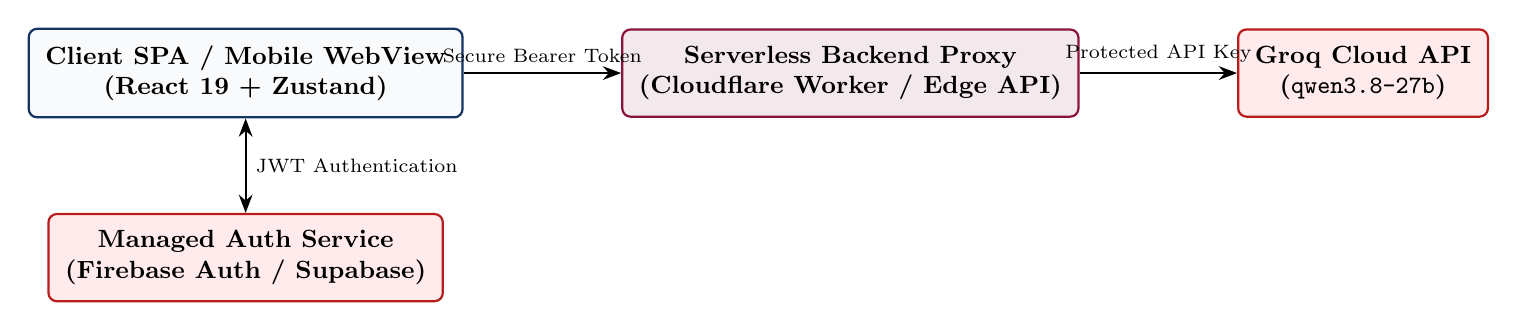
\begin{tikzpicture}[
    node distance=1.2cm and 1.8cm,
    clientBox/.style={rectangle, draw=primaryBlue, fill=lightBg, rounded corners=3pt, thick, align=center, font=\small\bfseries, inner sep=6pt},
    serverBox/.style={rectangle, draw=primaryMaroon, fill=primaryMaroon!10!white, rounded corners=3pt, thick, align=center, font=\small\bfseries, inner sep=6pt},
    extBox/.style={rectangle, draw=critRed, fill=red!8!white, rounded corners=3pt, thick, align=center, font=\small\bfseries, inner sep=6pt},
    >=Stealth, thick
]

\node[clientBox] (client) {Client SPA / Mobile WebView \\ (React 19 + Zustand)};
\node[serverBox, right=2cm of client] (proxy) {Serverless Backend Proxy \\ (Cloudflare Worker / Edge API)};
\node[extBox, right=2cm of proxy] (groq) {Groq Cloud API \\ (\texttt{qwen3.8-27b})};
\node[extBox, below=1.2cm of client] (auth) {Managed Auth Service \\ (Firebase Auth / Supabase)};

\draw[->] (client) -- node[above, font=\scriptsize] {Secure Bearer Token} (proxy);
\draw[->] (proxy) -- node[above, font=\scriptsize] {Protected API Key} (groq);
\draw[<->] (client) -- node[right, font=\scriptsize] {JWT Authentication} (auth);

\end{tikzpicture}
\caption{Target Production Architecture with Serverless Mediation}
\label{fig:target_arch}
\end{figure}

% =============================================================================
\chapter{Open Questions for Stakeholders}
% =============================================================================

\begin{table}[htbp]
\centering
\small
\caption{Audit Inquiries for Project Leadership}
\begin{tabularx}{\textwidth}{c X c l}
\toprule
\textbf{\#} & \textbf{Operational / Technical Inquiry} & \textbf{Status} & \textbf{Addressee} \\
\midrule
1 & Are the hardcoded API keys in \texttt{test\_*.cjs} active? Revocation required immediately. & \unknown & Project Lead \\
2 & Has Groq free-tier rate-limiting occurred during hackathon evaluations? & \unknown & Project Lead \\
3 & Was the web application deployed to public hosting or only distributed as an APK? & \unknown & Project Lead \\
4 & Were ``280+ peer-reviewed archives'' an intended future feature or pitch hyperbole? & \unknown & Presentation Author \\
5 & Is there an active engineering roadmap to implement real facial blurring and EXIF stripping? & \unknown & Tech Lead \\
6 & Did the root test scripts escape into committed public git history? & \unknown & Repository Admin \\
\bottomrule
\end{tabularx}
\end{table}

% =============================================================================
\appendix
% =============================================================================

\chapter{Full Repository File Inventory}

\begin{longtable}{p{5.5cm} p{10.5cm}}
\caption{Complete Codebase File Inventory} \label{tab:app_files} \\
\toprule
\textbf{File / Path} & \textbf{Description \& Audit Assessment} \\
\midrule
\endfirsthead
\caption[]{Complete Codebase File Inventory (Continued)} \\
\toprule
\textbf{File / Path} & \textbf{Description \& Audit Assessment} \\
\midrule
\endhead
\bottomrule
\endfoot
\texttt{.env} & Configuration containing Gemini and Groq API keys. \\
\texttt{.gitignore} & Git ignore rules including \texttt{.env}, \texttt{node\_modules}, and \texttt{dist}. \\
\texttt{.oxlintrc.json} & OxLint configuration with React and TypeScript plugins. \\
\texttt{Baseera\_Presentation\_Guide.txt} & Complete hackathon pitch script and slide presentation notes. \\
\texttt{Baseera\_Project\_and\_Presentation\_Guide.pdf} & Formatted PDF presentation guide. \\
\texttt{README.md} & Generic Vite boilerplate template README. \\
\texttt{baseera.apk} & Pre-built compiled Android APK (5.9 MB). \\
\texttt{baseera\_qrcode.png} & Distribution QR code linking to external download host. \\
\texttt{build\_final\_presentation\_pdf.py} & Python helper script for PDF generation. \\
\texttt{capacitor.config.ts} & Capacitor configuration for Android app packaging. \\
\texttt{generate\_pdf\_guide.py} & Python utility script for report compilation. \\
\texttt{index.html} & Application HTML entry point loading Google fonts and icons. \\
\texttt{package.json} & NPM package manifest declaring dependencies and build scripts. \\
\texttt{package-lock.json} & Exact dependency tree lockfile. \\
\texttt{postcss.config.js} & PostCSS configuration with TailwindCSS and Autoprefixer. \\
\texttt{tailwind.config.js} & Design system defining Material Design 3 tokens. \\
\texttt{test\_capabilities.cjs} & Diagnostic script for API feature probing. \\
\texttt{test\_gemini.cjs} & Gemini API diagnostic test with exposed key. \\
\texttt{test\_gemini2.cjs} & Extended Gemini test script. \\
\texttt{test\_groq.cjs} & Groq API diagnostic test with exposed key. \\
\texttt{test\_groq2.cjs} & Extended Groq test script. \\
\texttt{test\_image.cjs} & Multimodal vision API test script. \\
\texttt{test\_models.cjs} & LLM model comparison script. \\
\texttt{tsconfig.json} & Root TypeScript project configuration. \\
\texttt{tsconfig.app.json} & Application TypeScript configuration (ES2023, JSX). \\
\texttt{tsconfig.node.json} & Tooling TypeScript configuration. \\
\texttt{vite.config.ts} & Vite bundler and Vitest test runner configuration. \\
\texttt{src/main.tsx} & Application mount entry point. \\
\texttt{src/App.tsx} & React Router v7 configuration and authentication guard. \\
\texttt{src/store.ts} & State singleton and \texttt{localStorage} data bridge. \\
\texttt{src/index.css} & Global Tailwind stylesheet and design tokens. \\
\texttt{src/services/gemini.ts} & AI inference service connecting to Groq Cloud API. \\
\texttt{src/components/BottomNav.tsx} & Persistent mobile bottom navigation bar. \\
\texttt{src/screens/SplashScreen.tsx} & Launch screen with brand splash and auto-routing. \\
\texttt{src/screens/OnboardingScreen.tsx} & Three-slide tutorial carousel. \\
\texttt{src/screens/LoginScreen.tsx} & Credential authentication and guest access. \\
\texttt{src/screens/SignupScreen.tsx} & Registration screen with plaintext storage. \\
\texttt{src/screens/HomeScreen.tsx} & Main dashboard displaying recent analysis history. \\
\texttt{src/screens/ShareScreen.tsx} & Content ingestion interface (URL, upload, drag/drop). \\
\texttt{src/screens/ProcessingScreen.tsx} & Inference progress animation and API orchestration. \\
\texttt{src/screens/ResultScreen.tsx} & Analysis output display with bias gauge and pause timer. \\
\texttt{src/screens/PrivacyScreen.tsx} & Simulated Privacy Shield inspection interface. \\
\texttt{src/screens/ReportsScreen.tsx} & Weekly report dashboard with hardcoded statistics. \\
\texttt{src/test/setup.ts} & Vitest global mock setup. \\
\texttt{src/test/gemini.test.ts} & 20 unit tests for AI inference and fallback cascade. \\
\texttt{src/test/store.test.ts} & 16 unit tests for observation state and storage limits. \\
\texttt{src/test/auth.test.tsx} & 13 integration tests for authentication workflows. \\
\texttt{docs/PROJECT\_AUDIT.md} & Complete Markdown audit report source document. \\
\texttt{docs/baseera\_system\_architecture.tex} & LaTeX system architecture specification document. \\
\texttt{docs/baseera\_system\_architecture.pdf} & Compiled system architecture PDF. \\
\end{longtable}

\chapter{Audit Commands and Empirical Verification}

\begin{table}[htbp]
\centering
\small
\caption{Empirical Audit Execution Summary}
\begin{tabularx}{\textwidth}{l c X}
\toprule
\textbf{Executed Command} & \textbf{Exit Code} & \textbf{Empirical Execution Summary} \\
\midrule
\texttt{npx vitest run} & 0 & 3 test files, 49 tests executed, 49 passed in 30.28s. All fallback branches verified. \\
\addlinespace
\texttt{npx oxlint} & 1 & 1,841 warnings, 35 errors detected across 31 files. Primary errors: inline component recreation, cascading state calls in effects. \\
\bottomrule
\end{tabularx}
\end{table}

\chapter{Technical Glossary}

\begin{table}[htbp]
\centering
\small
\caption{Glossary of Technical and Pedagogical Terminology}
\begin{tabularx}{\textwidth}{l X}
\toprule
\textbf{Term} & \textbf{Definition} \\
\midrule
\textbf{Baseera} & Arabic word meaning ``insight,'' ``clear vision,'' or deep discernment. \\
\textbf{Socratic Prompting} & Pedagogical method using targeted probing inquiries rather than asserting direct factual verdicts. \\
\textbf{Cognitive Pause} & Deliberate temporal friction designed to disrupt System 1 reflexive social sharing loops. \\
\textbf{Groq LPU} & Language Processing Unit hardware providing low-latency inference for open models. \\
\textbf{Qwen 2.5 27B} & Alibaba open-weight large language model used for content bias evaluation. \\
\textbf{Capacitor} & Cross-platform runtime wrapping web applications into native iOS and Android shells. \\
\textbf{OxLint} & High-performance JavaScript/TypeScript linter written in Rust. \\
\textbf{BFF Layer} & Backend-for-Frontend architectural pattern mediating between client and upstream APIs. \\
\textbf{EXIF Data} & Metadata embedded in photographic files including GPS coordinates and camera specifications. \\
\bottomrule
\end{tabularx}
\end{table}

\chapter{Audit Scope and Coverage Checklist}

\begin{table}[htbp]
\centering
\small
\caption{Audit Scope and Verification Coverage}
\begin{tabularx}{\textwidth}{l c X}
\toprule
\textbf{Codebase Subsystem} & \textbf{Audit Depth} & \textbf{Verification Notes} \\
\midrule
\texttt{src/} Core Files & Full Line-by-Line & \texttt{main.tsx}, \texttt{App.tsx}, \texttt{store.ts}, \texttt{index.css} thoroughly audited. \\
\texttt{src/services/} & Full Line-by-Line & All 267 lines of \texttt{gemini.ts} analyzed. \\
\texttt{src/screens/} (10 Views) & Full Line-by-Line & All 10 screen components completely reviewed. \\
\texttt{src/test/} (3 Suites) & Full Line-by-Line & All 49 tests reviewed and executed. \\
Root Configuration & Full Line-by-Line & \texttt{package.json}, \texttt{vite.config.ts}, \texttt{tsconfig*.json} audited. \\
Root Diagnostics & Evidence-Checked & \texttt{test\_*.cjs} reviewed for hardcoded secret exposure. \\
Mobile Subsystem & Structural Review & Capacitor configuration and Android manifest verified. \\
\bottomrule
\end{tabularx}
\end{table}

\vspace{1cm}
\begin{center}
\itshape\small
--- End of Technical Audit Report --- \\
Report compiled on October 13, 2026. All findings verified against local repository sources.
\end{center}

\end{document}
